\color{blue}

\begin{figure*}[htbp]
    \centering
    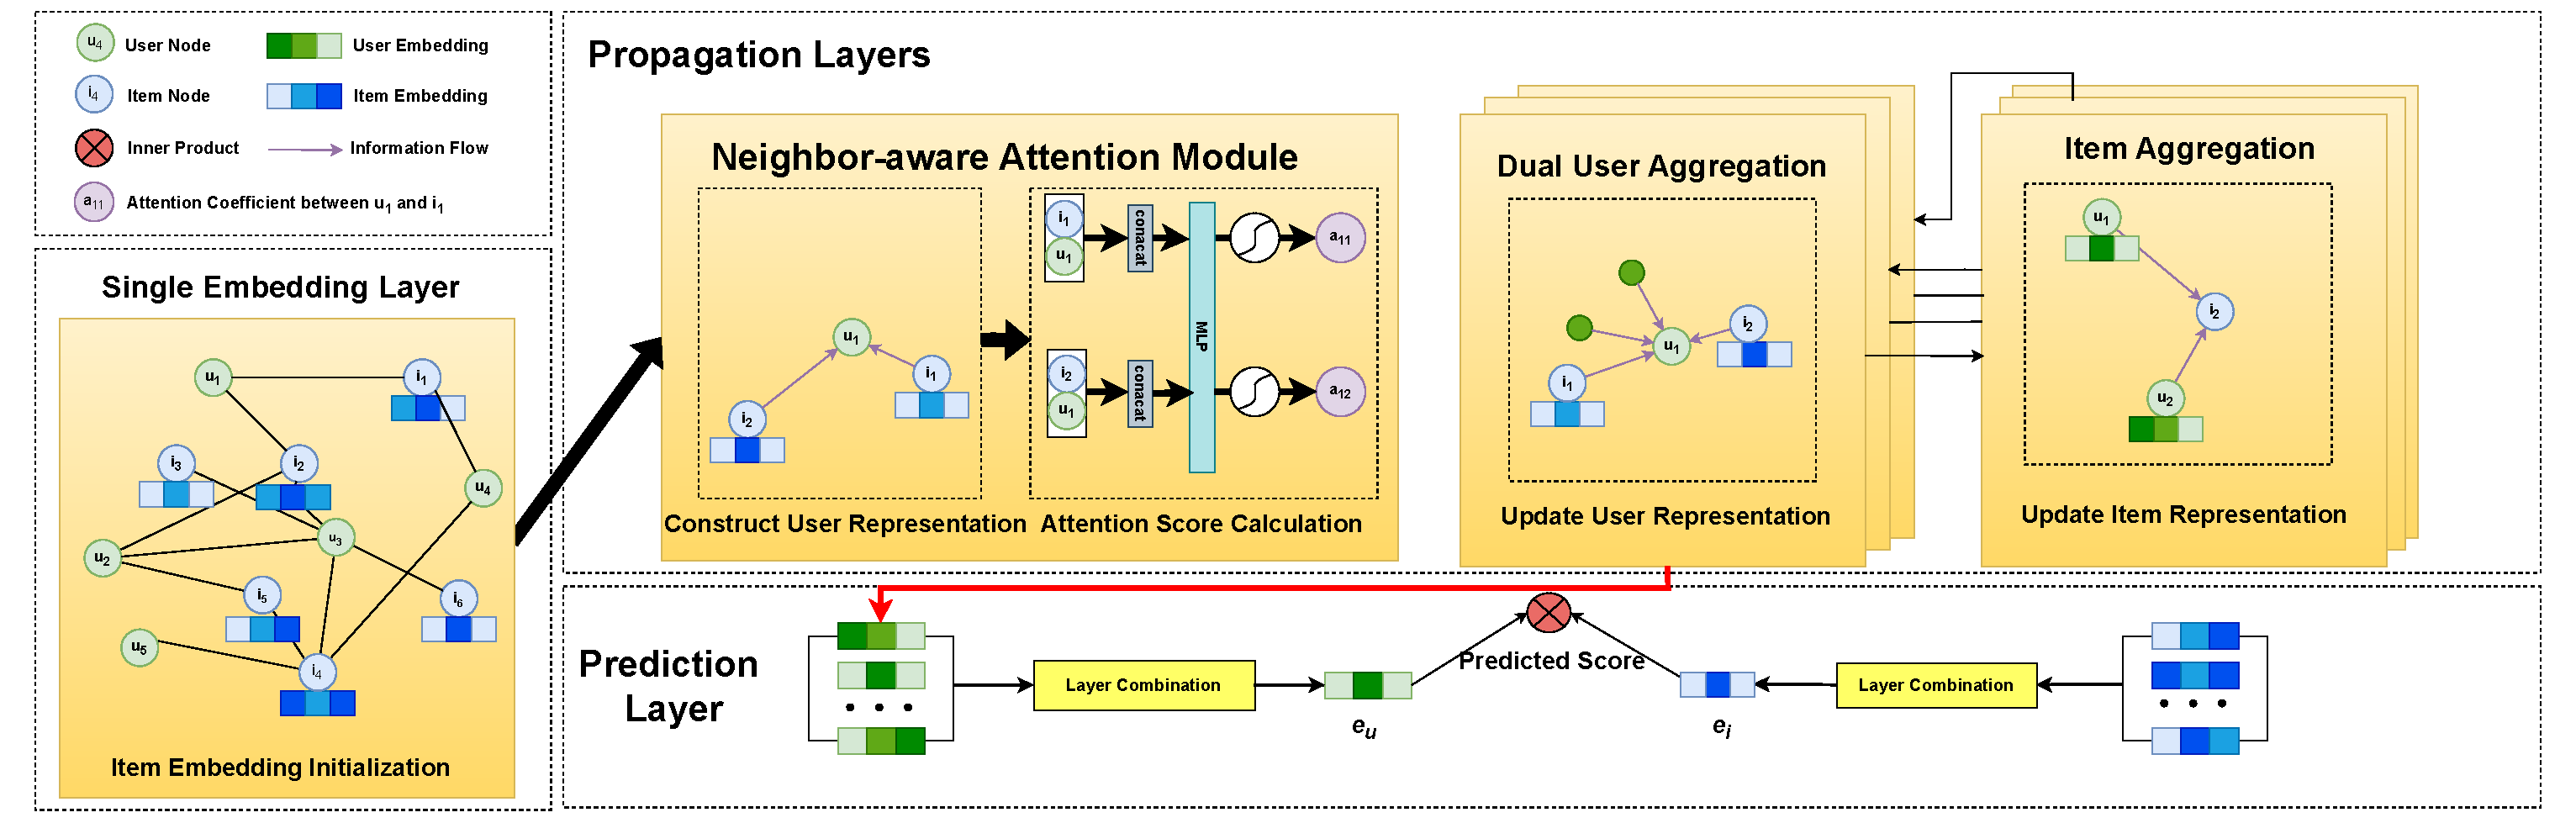
\includegraphics[width=\textwidth]{img/Model.pdf} % 替換成你的圖片檔案
    \caption{模型架構圖}
    \label{fig:cross-column}
\end{figure*}

\section{Proposed}
\subsection{Single Embedding Layer}
    本研究所採用的NIE-GCN\cite{NIE-GCN}~模型可拆解成幾個主要步驟,首先是對餐廳節點進行向量嵌入。第一步會針對每個餐廳節點 $i$ 生成一個嵌入向量 $e_i$,此向量位於 $d$ 維空間中,即 $e_i \in \mathbb{R}^d$。在嵌入過程中,所有餐廳節點的嵌入向量會被收集成一組矩陣 $E_I^{(0)}$,此矩陣表達了所有餐廳節點的初始嵌入狀態,如下式所示: 
    \begin{equation} 
        E_I^{(0)} = {e_{i_1}^{(0)}, e_{i_2}^{(0)},\cdots,e_{i_N}^{(0)}} \in \mathbb{R}^{N \times d}, 
    \end{equation}
    其中,$N$ 代表餐廳節點的總數,而 $d$ 則是嵌入向量的維度;上標 $0$ 表示第 0 層傳播的初始狀態。藉由得到每個餐廳節點的嵌入向量後,模型便可利用這些向量作為基礎,來進一步推斷每位使用者的偏好。因為每個使用者節點 $u$ 的鄰居必定為餐廳節點,故模型會透過與該使用者互動過的餐廳節點來推敲其個人喜好。

    在完成餐廳節點的嵌入後,第二步則是建構每位使用者節點的初始嵌入向量 $e_u^{(0)}$。此過程需要依賴與使用者節點 $u$ 相鄰的餐廳節點 $i$ 的嵌入向量 $e_i^{(0)}$。第 0 層的嵌入構造方式如下: 
    \begin{equation} 
        e_u^{(0)} = \sigma \left(\sum_{i \in N_u} \frac{1}{\sqrt{\vert N_u \vert \vert N_i \vert}}e_i^{(0)}\right), 
        \label{eq-e_u^0}
    \end{equation} 
    其中 $N_u$ 表示使用者節點 $u$ 的鄰居集合,而 $N_i$ 則代表餐廳節點 $i$ 的鄰居集合;$\sigma(\cdot)$ 是激活函數,選擇使用雙曲正切函數 (tanh)。透過這一層的加權平均,可以有效地融合使用者與其鄰近餐廳節點的特徵信息,以更準確地反映該使用者的行為特徵。

\subsection{Propagation Layers}
    完成初始嵌入後,下一步是計算每個使用者節點 $u$ 與其相鄰的餐廳節點 $i$ 之間的注意力分數 $\rho(u, i)$,藉此衡量不同鄰居節點的重要性。該分數計算方式如下: 
    \begin{equation} 
        \rho(u, i) = Q^T\sigma(W(e_u^{(0)}||(e_i^{(0)})+b)), 
    \end{equation} 
    其中 $W \in \mathbb{R}^{2d \times d}$、$Q \in \mathbb{R}^{1 \times d}$、$b \in \mathbb{R}^{1 \times d}$,這三個參數分別為注意力機制中的權重矩陣與偏置項。此處的 $\sigma(\cdot)$ 同樣為雙曲正切函數 (tanh),而 $||$ 則表示向量的串接操作。$\rho(u, i)$ 的分數越高,代表使用者 $u$ 與餐廳 $i$ 之間的關聯性越強。因此,透過該分數可以量化每個餐廳節點對於預測使用者偏好的貢獻度。

    為將注意力分數限制在 $[0,1]$ 的範圍內,利用 Softmax 函數對這些分數進行範圍歸一化處理,得到最終的注意力值 $\alpha(u, i)$。公式如下: \begin{equation} \alpha(u, i) = \frac{\exp(\rho(u, i))}{\left(\sum_{j \in N_u}\exp(\rho(u, j))\right)^{\beta}}. \end{equation} 其中 $\alpha(u, i)$ 代表了使用者節點 $u$ 與餐廳節點 $i$ 之間的最終注意力值。透過~$\alpha(u, i)$,每個使用者節點均能依據其鄰居的特徵,綜合考量注意力分數來完成向量更新。


    在初始嵌入狀態完成後,為進行更深層的特徵傳播,使用者節點 $u$ 的嵌入向量 $e_u^{(k)}$ 將在每一層根據其鄰居節點的資訊進行更新。使用者的嵌入向量 $e_u^{(k)}$ 的更新方式會依據先前計算出的注意力權重 $\alpha(u, i)$,並利用相鄰餐廳節點 $i$ 在上一層的嵌入向量 $e_i^{(k-1)}$ 進行加法聚合 (Add Aggregation)。此聚合方式可以有效融合鄰居的特徵信息,更新的計算公式如下: 
    \begin{equation} 
        e_u^{(k)} = \sigma\left(\sum_{i \in N_u} \alpha(u, i)e_i^{(k-1)}\right), 
    \end{equation} 
    其中,$\sigma(\cdot)$ 為雙曲正切函數 (tanh),$N_u$ 表示使用者節點 $u$ 的鄰居集合。透過加權聚合,使用者節點可以自適應地調整對不同鄰居特徵的重視程度,進一步增強模型對於不同使用者偏好的捕捉能力。

    同樣地,初始狀態後的餐廳節點的嵌入向量 $e_i^{(k)}$ 也會根據其相鄰使用者節點的嵌入進行更新。這個更新方式與\xeq{eq-e_u^0}~類似,餐廳節點 $i$ 的嵌入向量會根據其相鄰的使用者節點 $u$ 的嵌入向量 $e_u^{(k)}$ 進行加權平均,計算方式如下: 
    \begin{equation} e_i^{(k)} = \sigma \left(\sum_{u \in N_i} \frac{1}{\sqrt{\vert N_u \vert \vert N_i \vert}} e_u^{(k)}\right), 
        \label{eq-e_i} 
    \end{equation} 其中,$N_u$ 和 $N_i$ 分別表示使用者節點 $u$ 和餐廳節點 $i$ 的鄰居集合,並透過加權平均來控制每個鄰居對於嵌入向量的貢獻。此\xeq{eq-e_i}~與\xeq{eq-e_u^0}~中的加權項 $\frac{1}{\sqrt{\vert N_u \vert \vert N_i \vert}}$ 可以平衡不同鄰居數量對嵌入更新的影響,從而避免由於鄰居數量不均而引起的偏差。藉由此加權項,每個餐廳節點的嵌入向量都將根據與其相鄰使用者的特徵進行有效更新,從而更準確地反映餐廳與使用者間的潛在關係。

\subsection{Prediction Layers}
    在完成每一層使用者節點的嵌入向量 $e_u^{(k)}$ 和餐廳節點的嵌入向量 $e_i^{(k)}$ 的計算後,接下來的步驟是將這些嵌入向量進行聚合,以獲得最終的嵌入表達,在本研究將所有層的使用者嵌入向量和餐廳嵌入向量分別相加,計算公式如下: 
    \begin{equation} 
        e_u^* = \sum_{k=1}^{L} e_u^{(k)}, \quad e_i^* = \sum_{k=1}^{L} e_i^{(k)}, 
    \end{equation} 
    其中 $L$ 表示嵌入層的總數。這樣計算得到的 $e_u^*$ 和 $e_i^*$ 分別代表了使用者節點和餐廳節點的最終嵌入向量,這兩個向量綜合了多層的信息,能夠更全面地捕捉使用者與餐廳之間的潛在關聯。
    為了進一步評估使用者 $u$ 和餐廳 $i$ 之間的關聯性,將這兩個最終嵌入向量進行內積操作,為了將內積值限制在 0 到 1 的範圍內,引入了 S 型函數 (sigmoid function),計算公式如下: 
    \begin{equation} 
        \hat{y_{ui}} = f(u, i) = \sigma(e_u^{T} e_i^), 
    \end{equation} 
    其中,$\hat{y_{ui}}$ 表示模型對於使用者 $u$ 和餐廳 $i$ 之間關聯性的預測結果。S 型函數 $\sigma(\cdot)$ 將內積的結果映射到 $[0, 1]$ 的範圍,使得模型的輸出可以被解釋為一個概率值,表達使用者 $u$ 對餐廳 $i$ 的喜好程度。

\subsection{Model Optimization}
    待完成
